\documentclass[11pt,a4paper]{article}

% For å kunne skrive norske tegn.
\usepackage[utf8]{inputenc}

% For å inkludere figurer.
\usepackage{graphicx}

% Ekstra matematikkfunksjoner.
\usepackage{amsmath,amssymb}

\usepackage{hyperref}
\usepackage{fancyvrb}

\newenvironment{code}
  {
    \VerbatimEnvironment
    \vskip\baselineskip\hrule
    \begin{Verbatim}[xleftmargin=7pt]%
  }
  {\end{Verbatim}\hrule\vskip\baselineskip}

% Må inkluderes for blant annet å få tilgang til kommandoen \SI (korrekte måltall med enheter)
\usepackage{siunitx}

  % Prikk som multiplikasjonstegn (i steden for kryss).
  \sisetup{exponent-product = \cdot}

  % Pluss-minus-form på usikkerhet (i steden for parentes).
  \sisetup{separate-uncertainty = true}

% For å få tilgang til finere linjer (til bruk i tabeller og slikt).
\usepackage{booktabs}

% For justering av figurtekst og tabelltekst.
\usepackage[font=small,labelfont=bf]{caption}

% Subsections A, B,
\renewcommand{\thesubsection}{\Alph{subsection}}

% Disse kommandoene kan gjøre det enklere for LaTeX å plassere figurer og tabeller der du ønsker.
\setcounter{totalnumber}{5}
\renewcommand{\bottomfraction}{0.95}
\renewcommand{\floatpagefraction}{0.35}

\begin{document}

  % Rapportens tittel:
  \title{Lab 5: Information Access \\ \large{TDT4275: Natural Language Interfaces}}
  \author{Jonas Myrlund}

  % Her ber vi LaTeX om å lage tittelen (til nå har vi bare sagt hva den skal inneholde):
  \maketitle

  \section{Written Assignments} % (fold)
  \label{sec:written_assignments}

    \subsection{Using either web searches or a large corpus, devise a query using a polysemous word.} % (fold)
    \label{sub:using_either_web_searches_or_a_large_corpus_devise_a_query_using_a_polysemous_word_}

      I want to find out more about large cranes -- the bird. I start out with the following query:
      ``large crane''.

      See figure \ref{fig:large_crane_google} for the initial results using Google\footnote{\url{https://google.com/search?q=large+crane}}.

      \begin{figure}
        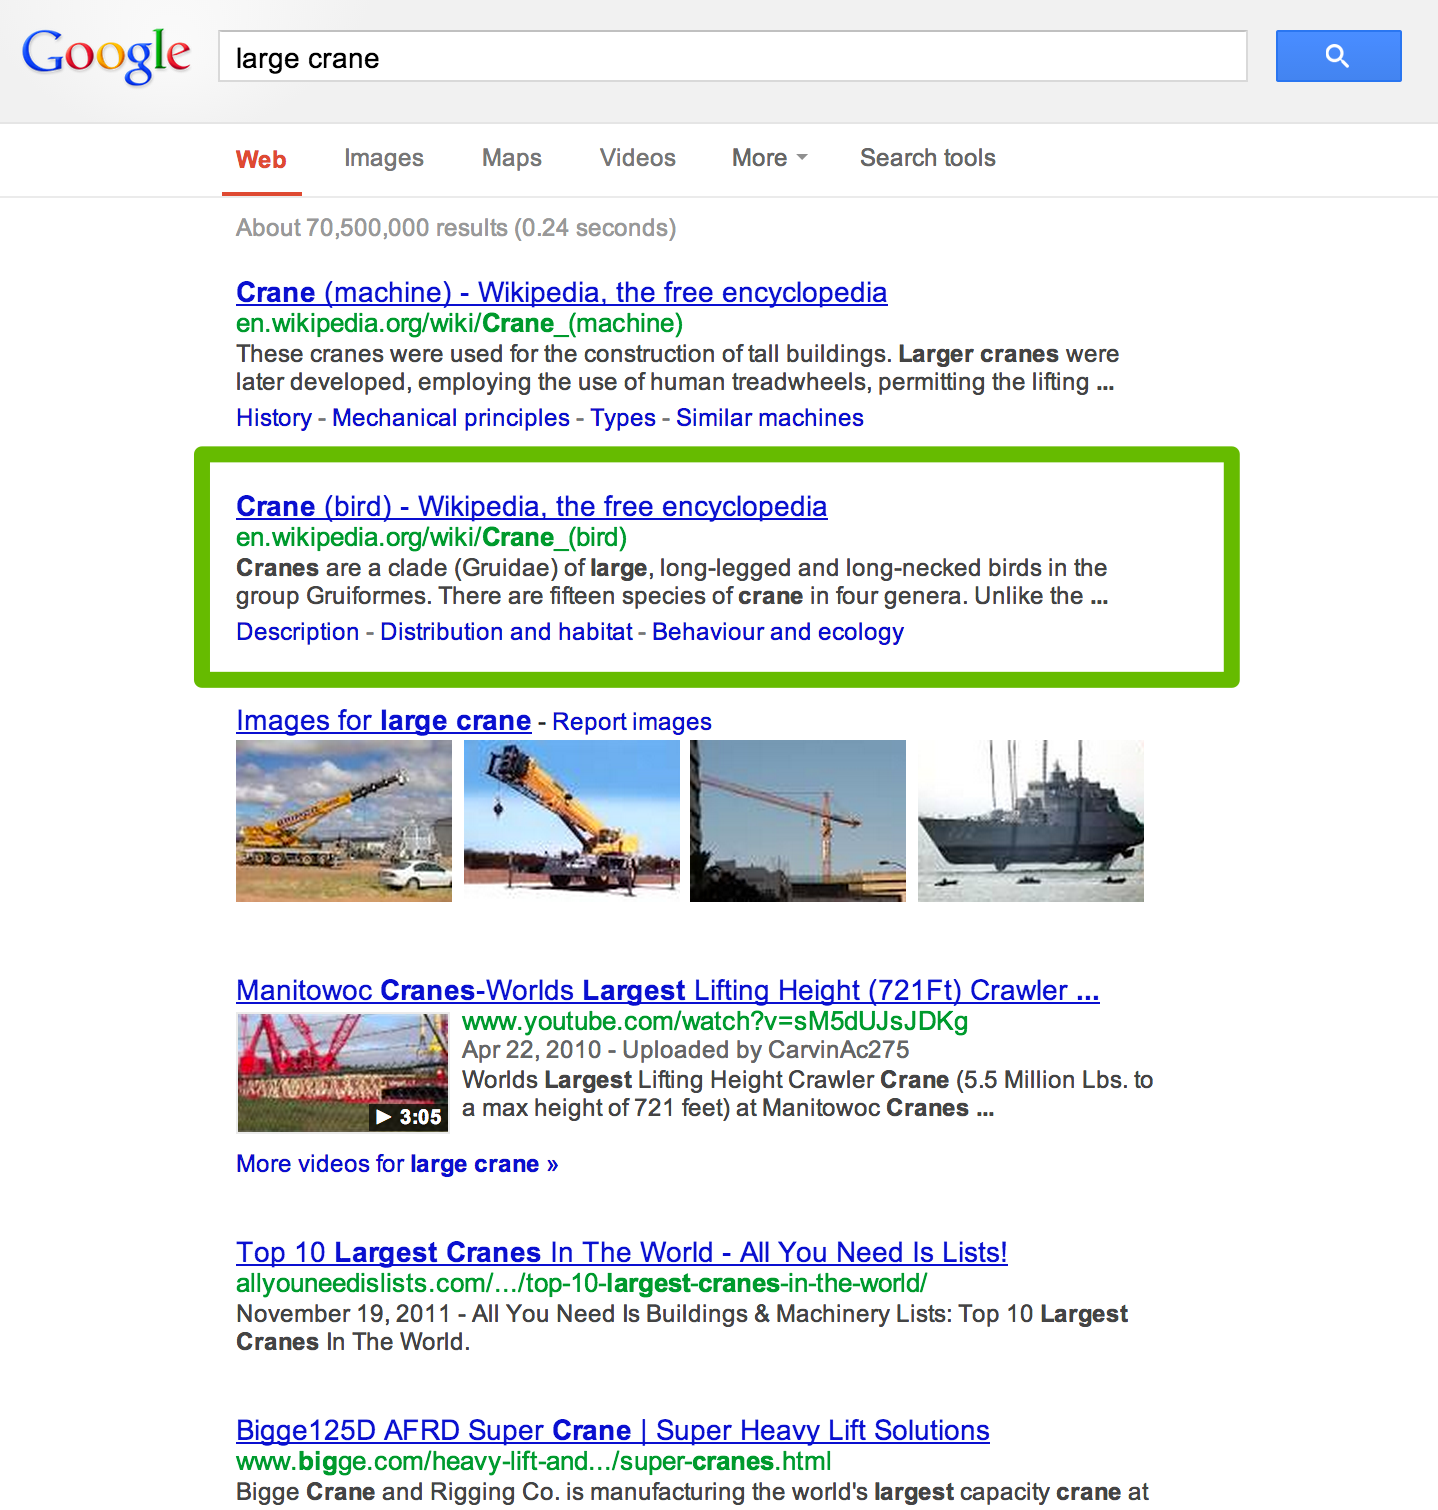
\includegraphics[width=0.95\textwidth]{imgs/large_crane_google}
        \caption{Google yields only one relevant search result when searching for ``large crane''.}
        \label{fig:large_crane_google}
      \end{figure}

    % subsection using_either_web_searches_or_a_large_corpus_devise_a_query_using_a_polysemous_word_ (end)

    \subsection{Then, devise two or three alternate queries which help to disambiguate the polysemous word and repeat the search.} % (fold)
    \label{sub:then_devise_two_or_three_alternate_queries_which_help_to_disambiguate_the_polysemous_word_and_repeat_the_search_}

      The query ``large crane'' could be less ambiguous in the following ways:

      \begin{enumerate}
        \item ``large crane bird''
        \item ``large crane feathers''
      \end{enumerate}

      As figure \ref{fig:large_crane_bird_google} exemplifies, these queries result in only documents relating to the \emph{bird sense} of the word \emph{crane}.

      \begin{figure}
        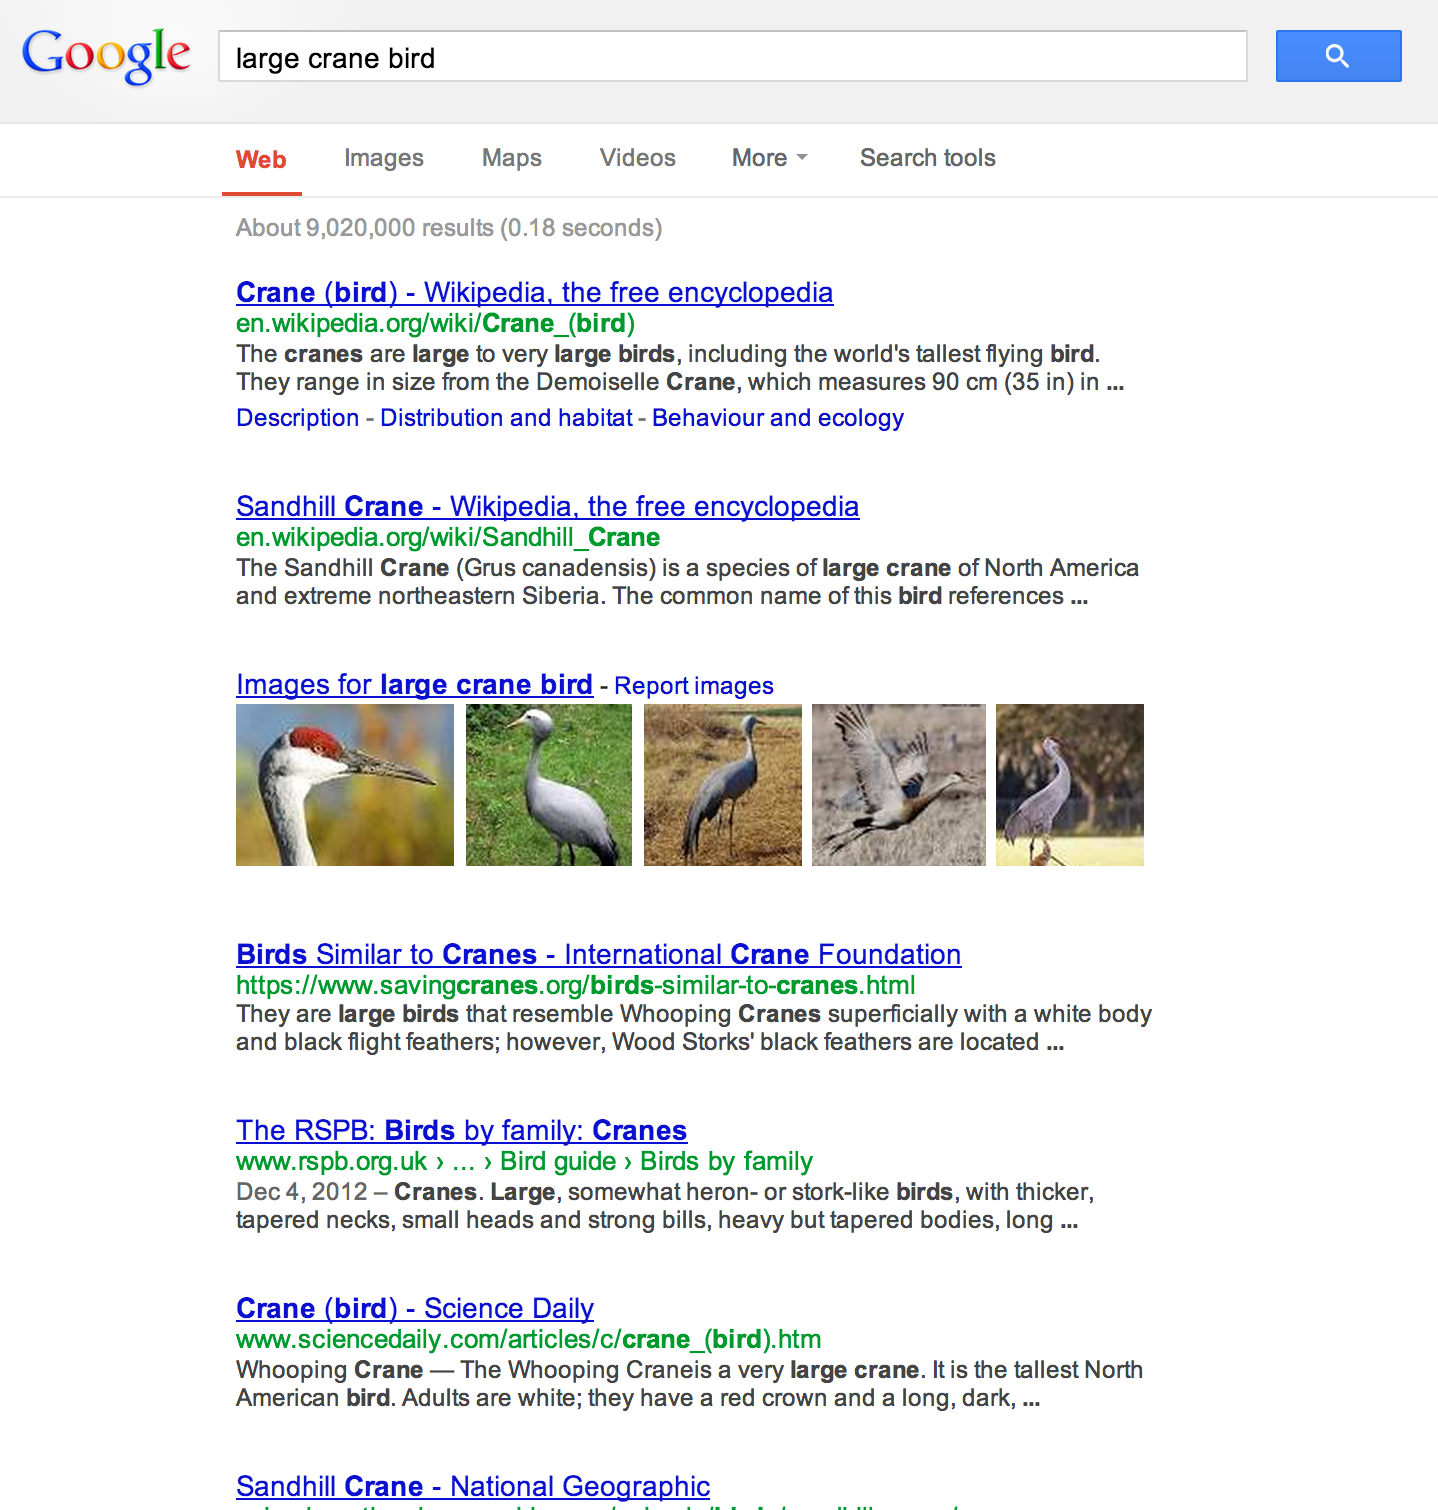
\includegraphics[width=0.95\textwidth]{imgs/large_crane_bird_google}
        \caption{When adding the term ``bird'' to the query, all the top results are relevant.}
        \label{fig:large_crane_bird_google}
      \end{figure}

    % subsection then_devise_two_or_three_alternate_queries_which_help_to_disambiguate_the_polysemous_word_and_repeat_the_search_ (end)

    \subsection{For each query, classify each of the top 10 search results as correct or incorrect.} % (fold)
    \label{sub:for_each_query_classify_each_of_the_top_10_search_results_as_correct_or_incorrect_}

      Again, I will be using Google for the queries.

      \subsubsection{Query: ``large crane''} % (fold)
      \label{ssub:query_large_crane_}

        The query yields only one correct document: the second search result.
        The others documents relate to the wrong sense of the word.
        For details, see figure \ref{fig:large_crane_google}.

      % subsubsection query_large_crane_ (end)

      \subsubsection{Queries: ``large crane bird'' and ``large crane feathers''} % (fold)
      \label{ssub:query_large_crane_bird_}

        For both these queries, all the first 10 search results relate to the right sense of the polysemous word in Google.

        Yahoo! and Bing, however, both give three documents relating only to feathers, which is not what is wanted.

      % subsubsection query_large_crane_bird_ (end)

    % subsection for_each_query_classify_each_of_the_top_10_search_results_as_correct_or_incorrect_ (end)

    \subsection{Create an interpolated precision-recall curve comparing the accuracy of each of the queries.} % (fold)
    \label{sub:create_an_interpolated_precision_recall_curve_comparing_the_accuracy_of_each_of_the_queries_}

      The recall values for the first query, ``large crane'', stagnates in that it gives only one correct document.
      Thus, the scales of the precision-recall curves do not overlap to a degree that makes it viable to plot them together.

      However, the curves quite clearly show the improvement adding a disambiguating term yields, when the precision axis is normalized to one. See figure \ref{fig:pr1}, \ref{fig:pr2} and \ref{fig:pr3}.

      \begin{figure}[h]
        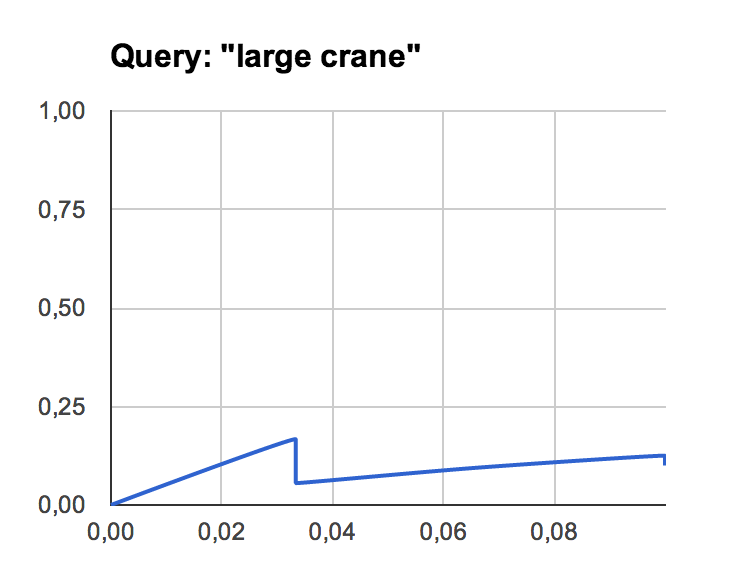
\includegraphics[width=0.85\textwidth]{imgs/large_crane_pr}
        \caption{Precision-recall curve for ``large crane''.}
        \label{fig:pr1}
      \end{figure}

      \begin{figure}[h]
        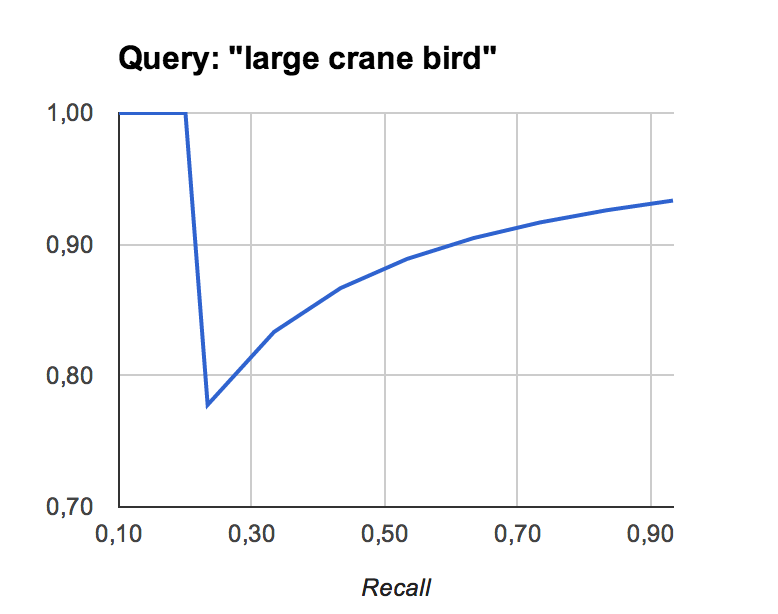
\includegraphics[width=0.85\textwidth]{imgs/large_crane_bird_pr}
        \caption{Precision-recall curve for ``large crane bird''.}
        \label{fig:pr2}
      \end{figure}

      \begin{figure}[h]
        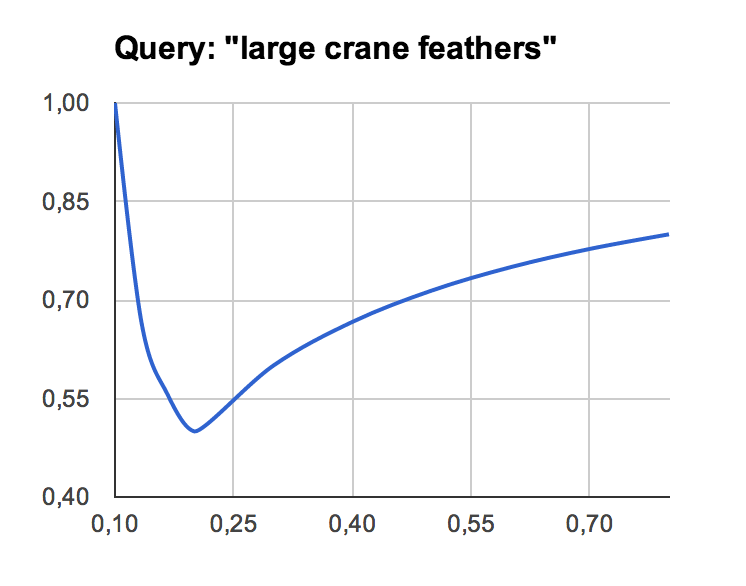
\includegraphics[width=0.85\textwidth]{imgs/large_crane_feathers_pr}
        \caption{Precision-recall curve for ``large crane feathers''.}
        \label{fig:pr3}
      \end{figure}

    % subsection create_an_interpolated_precision_recall_curve_comparing_the_accuracy_of_each_of_the_queries_ (end)

  % section written_assignments (end)

\end{document}















